\documentclass[11pt,a4paper]{article}
\usepackage[T1]{fontenc}
\usepackage[utf8]{inputenc}
\usepackage{lmodern}
\usepackage[margin=24mm]{geometry}
\usepackage{rotating}
\usepackage{tikz}
\usetikzlibrary{arrows.meta,positioning,calc,fit}
\usepackage{microtype}
\usepackage{amsmath,amssymb,bm}
\usepackage{booktabs,tabularx,array,longtable}
\usepackage{graphicx}
\usepackage{xcolor}
\usepackage{hyperref}
\definecolor{navy}{HTML}{17324D}
\definecolor{blue}{HTML}{246BFD}
\definecolor{teal}{HTML}{00A88F}
\definecolor{orange}{HTML}{F58B2A}
\definecolor{purple}{HTML}{7559D9}
\definecolor{light}{HTML}{F3F6FA}
\definecolor{mid}{HTML}{607089}
\hypersetup{colorlinks=true,linkcolor=navy,citecolor=teal,urlcolor=blue,pdftitle={Ball World Model: Architecture and Evaluation Reference},pdfauthor={Jasper Juchem}}
\newcommand{\R}{\mathbb{R}}\newcommand{\norm}[1]{\left\lVert #1\right\rVert}\newcommand{\E}{\mathbb{E}}\newcommand{\dt}{\Delta t}
\begin{document}
\begin{titlepage}
\centering
\vspace*{30mm}
{\Huge\bfseries\color{navy} Ball World Model}\\[4mm]
{\LARGE Architecture, Training Objectives, Representation Analysis, and \textbf{Translation-Only} Evaluation}\\[7mm]
{\textit{dr. Jasper Juchem}}\\[7mm]
{\color{blue}\rule{\textwidth}{2.2pt}}\\[12mm]
{\large A technical reference for machine-learning researchers}\\[20mm]
{\large\color{navy}\textbf{Idea:} RGB sequence $\rightarrow$ spatial features $\rightarrow$ content and motion $\rightarrow$ metric state}
\vfill
{\large Based on the \texttt{ball\_simulator} source tree and the successful translation-only evaluation dated 2026-08-27}\\[5mm]
{\small Version 1.0 -- 31 August 2026}
\end{titlepage}
\pagenumbering{roman}
\begin{abstract}
This report reconstructs the complete translation-only neural state-estimation pipeline implemented in the supplied project source. It explains the tensor geometry, coordinate-aware convolutional encoder, differentiable soft-keypoint bottleneck, content and motion representations, bidirectional latent transition, supervised state heads, iterative metric-space physics corrector, loss design, data protocol, and evaluation methodology. The central empirical observation is a strong representation split: static content is almost perfectly linearly informative about position, while temporal differences and the learned motion representation are strongly informative about velocity. The report distinguishes what is directly guaranteed by the implementation from what is an interpretation supported by probes and interventions. It also clarifies the model's status as a finite-window neural observer with one-step latent predictive structure rather than an autonomous long-horizon simulator.
\end{abstract}
\tableofcontents
\clearpage\pagenumbering{arabic}

\section{Scope, provenance, and terminology}
The primary source is the supplied code archive \texttt{eventBased\_worldModels-state\_estimates.zip}, including the \texttt{ball\_simulator/src/ball\_world\_model} package and translation experiment configuration. The empirical source is \texttt{evaluation\_260827.zip}. Numerical values in this document are taken from that evaluation. Literature citations are used to contextualize design patterns, not to substitute for code inspection.

Throughout, $B$ is batch size, $T$ is the number of frames in a context window, $H=W=256$, $C=128$ is the final feature-channel count, $K=8$ is the number of soft keypoints, $D_z=256$ is the content embedding dimension, and $D_m=256$ is the motion dimension. A hat denotes a prediction or estimate. Ground-truth metric states are denoted by a superscript $\mathrm{gt}$.

\begin{quote}\textbf{Executive model classification.} 
The implemented network is best described as a \textbf{visual neural state observer with a one-step joint-embedding latent transition}. It estimates position and velocity from observed image windows. It can predict the next content embedding locally, but it does not yet define a complete autonomous multi-step rollout because the motion representation is extracted from pairs of observed feature maps.
\end{quote}

\section{Problem formulation}
\subsection{Inputs, targets, and deployment contract}
For each sampled window, the network receives RGB images only:
\begin{equation}
\bm I_{1:T}\in\R^{B\times T\times 3\times256\times256},\qquad T=10.
\end{equation}
The simulator-provided position and velocity are training and evaluation targets,
\begin{equation}
\bm p^{\mathrm{gt}}_{1:T}\in\R^{B\times T\times3},\qquad
\bm v^{\mathrm{gt}}_{1:T}\in\R^{B\times T\times3},
\end{equation}
not inputs to the forward pass. There is no state-label encoder $E_x(\bm p,\bm v)$ and no target latent computed from numerical ground truth. At deployment, inference is therefore
\begin{equation}
\bm I_{1:T}\longmapsto(\widehat{\bm p}_{1:T},\widehat{\bm v}_{1:T}).
\end{equation}
The learned latent variables are visually induced internal coordinates. Metric supervision shapes their usefulness through the readout losses, but does not make them equal to the physical state.

\subsection{Sampling and temporal scale}
The translation configuration uses rendered \,100 Hz video, frame stride one, ten context frames, one prediction frame, and four target-history frames. Thus $\dt=0.01\,\mathrm{s}$ and the ten-frame context spans nine inter-frame intervals, or \,90 ms. The dataset is split 80/10/10 at a fixed seed; the data loader uses batch size 16.

\section{Architecture overview}
\begin{sidewaysfigure}[htbp]
	\centering
	%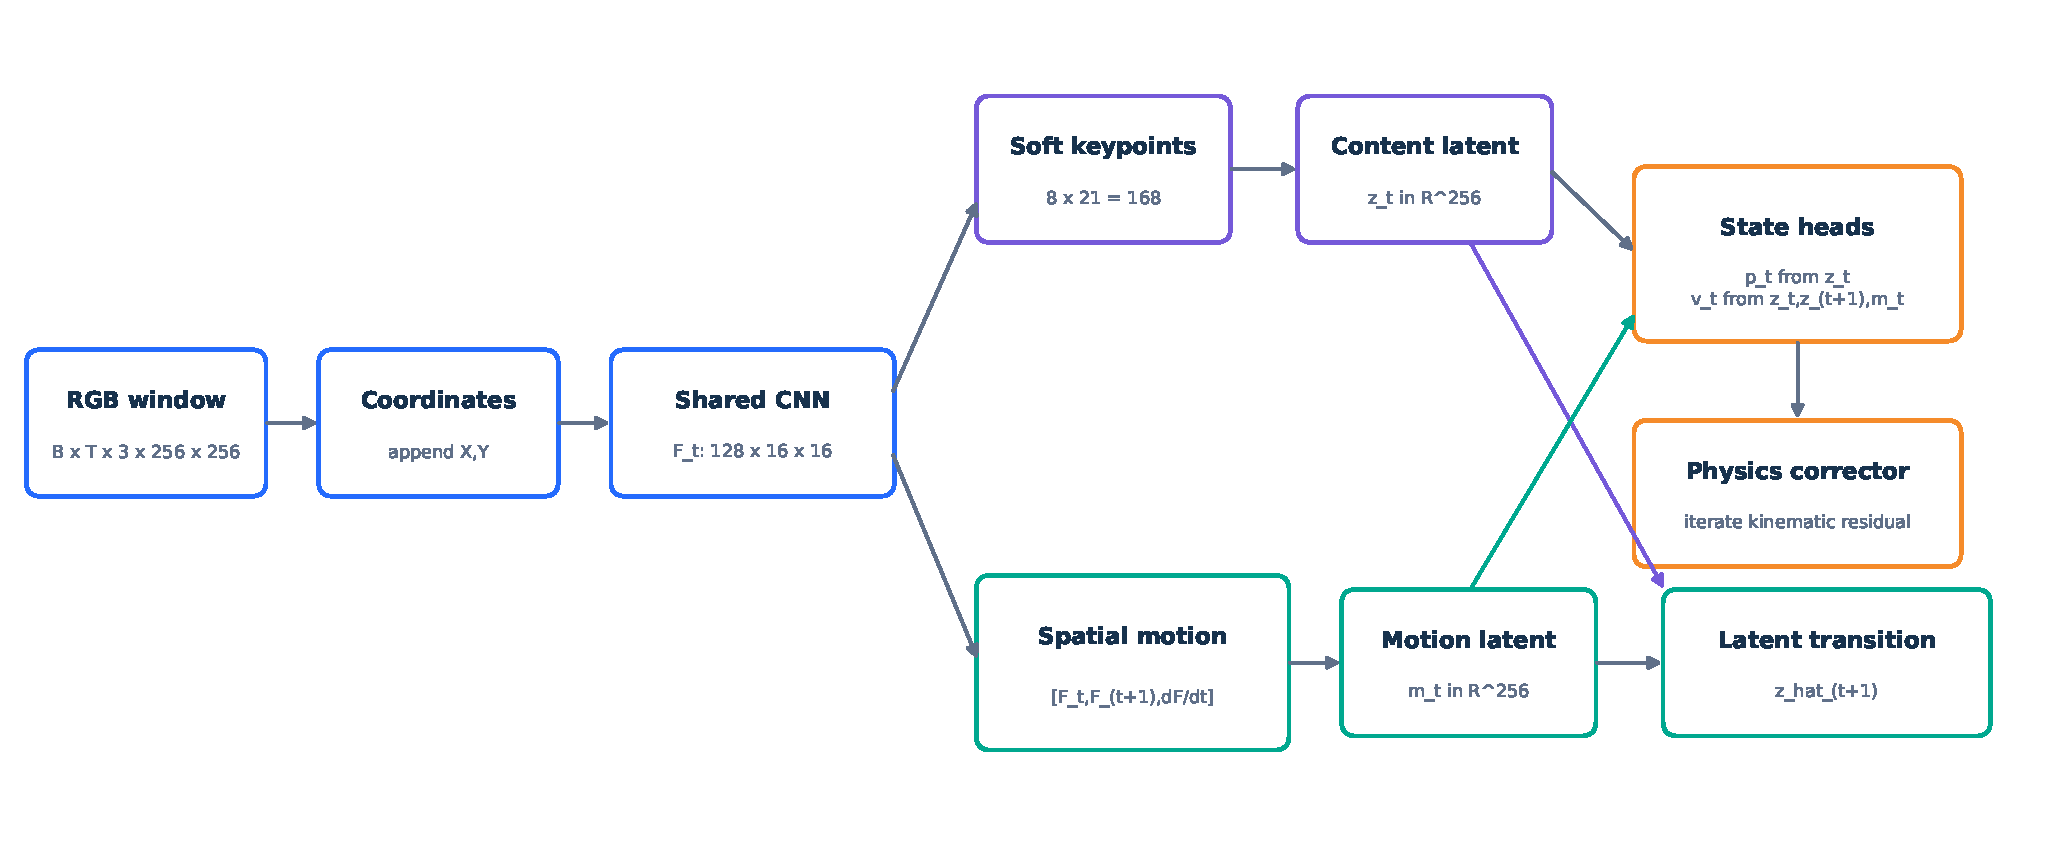
\includegraphics[width=\textwidth]{figures/architecture_overview.pdf}
	%\documentclass{article}
%% Requires in the parent document preamble:
%\usepackage{tikz}
%\usetikzlibrary{arrows.meta,positioning,calc,fit}
%\usepackage{amsmath,amssymb,bm}
%\usepackage{rotating}
%\begin{document}
%
%\begin{sidewaysfigure}
\begin{tikzpicture}[
  font=\small,
  >=Latex,
  box/.style={draw, rounded corners=2pt, align=center, minimum height=10mm,
              fill=white, inner sep=4pt},
  inference/.style={-{Latex}, thick, draw=black!65},
  target/.style={-{Latex}, thick, dashed, draw=purple!80!black},
  constraint/.style={-{Latex}, thick, dashed, draw=orange!90!black},
  supervision/.style={-{Latex}, thick, dashed, draw=blue!75!black}
]
% Inference graph
\node[box,draw=blue!75!black,fill=blue!5] (img)
  {$\mathbf I_{1:T}$\\ \tiny$B\times T\times3\times256\times256$};
\node[box,draw=blue!75!black,below=8mm of img] (coord)
  {append $X,Y$\\ \tiny5 input channels};
\node[box,draw=blue!75!black,below=8mm of coord] (feat)
  {shared CNN\\$\mathbf F_t\in\mathbb R^{128\times16\times16}$};

\node[box,draw=purple!75!black,above right=8mm and 8mm of feat] (kp)
  {8 soft keypoints\\168 statistics};
\node[box,draw=purple!75!black,right=5mm of kp] (z)
  {content latent\\$\mathbf z_t\in\mathbb R^{256}$};
\node[box,draw=purple!75!black,above=5mm of z] (znext)
  {observed target latent\\$\mathbf z_{t+1}=E_z(\mathbf F_{t+1})$};

\node[box,draw=teal!70!black,below right=8mm and 5mm of feat] (motion)
  {$[\mathbf F_t,\mathbf F_{t+1},\dot{\mathbf F}_t]$\\ \tiny spatial motion encoder};
\node[box,draw=teal!70!black,right=8mm of motion] (m)
  {motion latent\\$\mathbf m_t\in\mathbb R^{256}$};
\node[box,draw=teal!70!black,right=8mm of m] (transition)
  {latent transition\\$\widehat{\mathbf z}_{t+1}=\mathbf z_t+\Delta t\,T_\theta(\mathbf m_t)$};

\node[box,draw=orange!85!black,right=20mm of znext] (heads)
  {state heads\\$\widehat{\mathbf p}_t=h_p(\mathbf z_t)$\\
   $\widehat{\mathbf v}_t=h_v(\mathbf z_t,\mathbf z_{t+1},\mathbf m_t)$};
\node[box,draw=orange!85!black,below=8mm of heads] (corrector)
  {iterative metric corrector\\
   $\mathbf r_t=\widehat{\mathbf p}_{t+1}-\widehat{\mathbf p}_t
   -\Delta t\,\widehat{\mathbf v}_t$};

% Training-only nodes
\node[box,draw=purple!75!black,fill=purple!4,below=4mm of transition] (latentloss)
  {latent prediction loss\\
   $\mathcal L_{\mathrm{latent}}=\lVert\widehat{\mathbf z}_{t+1}-\mathbf z_{t+1}\rVert^2$};
\node[box,draw=blue!75!black,fill=blue!4,right=4mm of heads] (gt)
  {training targets only\\$\mathbf p_t^{\mathrm{gt}},\mathbf v_t^{\mathrm{gt}}$};
\node[box,draw=purple!75!black,fill=purple!4,below=7mm of gt] (stateloss)
  {state loss\\$\mathcal L_{\mathrm{state}}$};

% Solid inference paths
\draw[inference] (img)--(coord);
\draw[inference] (coord)--(feat);
\draw[inference] (feat)--(kp);
\draw[inference] (kp)--(z);
\draw[inference] (feat)--(motion);
\draw[inference] (motion)--(m);
\draw[inference] (m)--(transition);
\draw[inference] (z.south east) -- ++(5mm,-5mm) |- (transition.west);
\draw[inference] (znext.east) -- (heads.west);
\draw[inference] (z.east) -- ++ (15mm, 15mm) |- (heads.west);
\draw[inference] (m.north) -- ++ (0mm, 5mm) -- ++ (27mm, 0mm) |- (heads.west);
\draw[inference] (heads)--(corrector);

% Dashed learning targets and constraints
\draw[target] (transition.south) -- (latentloss.north);
\draw[target] (znext.south) |- (latentloss.west);
\draw[constraint] (heads.south east) -- node[pos=0.5,left,font=\scriptsize,align=left]
  {kinematic consistency\\and iterative refinement} (corrector.north east);
\draw[supervision] (heads.east) -- (stateloss.west);
\draw[supervision] (gt.south) -- (stateloss.north);

% Legend
\node[below left=45mm and 0mm of feat.south west,anchor=north west] (legend) {%
\begin{tikzpicture}[baseline]
  \draw[inference] (0,0)--(0.9,0); \node[right] at (0.95,0) {inference path};
  \draw[target] (3.5,0)--(4.4,0); \node[right] at (4.45,0) {learning target};
  \draw[constraint] (7.1,0)--(8.0,0); \node[right] at (8.05,0) {physics consistency};
  \draw[supervision] (11.0,0)--(11.9,0); \node[right] at (11.95,0) {ground-truth supervision};
\end{tikzpicture}};
\end{tikzpicture}
%\end{sidewaysfigure}
%\end{document}

	\caption{End-to-end computation graph. Solid lines are inference paths. Dashed lines indicate learning targets or consistency constraints.}
	\label{fig:overview}
\end{sidewaysfigure}

The architecture deliberately delays global compression. Each image is first transformed into a spatial tensor $\bm F_t$, from which two complementary descriptions are derived:
\begin{align}
\bm z_t &= E_z(\bm F_t), &&\text{content / configuration-like information},\\
\bm m_t &= E_m(\bm F_t,\bm F_{t+1},\dot{\bm F}_t), &&\text{motion / tangent-like information}.
\end{align}
The position head uses $\bm z_t$, while the velocity head receives the pair $(\bm z_t,\bm z_{t+1})$ and the interval motion embedding $\bm m_t$. A latent transition predicts adjacent content embeddings. A final iterative corrector enforces translational kinematic consistency in metric coordinates.

\section{Coordinate-aware frame encoder}
\subsection{Coordinate augmentation}
Two deterministic coordinate planes are appended to every RGB input. For pixel indices $(i,j)$,
\begin{equation}
X_{ij}=2\frac{j}{W-1}-1,\qquad Y_{ij}=2\frac{i}{H-1}-1.
\end{equation}

The backbone input is therefore
\begin{equation}
\widetilde{\bm I}_t=\operatorname{concat}(\bm I_t,\bm X,\bm Y)
\in\R^{5\times256\times256}.
\end{equation}
Ordinary convolution is translation equivariant and does not expose absolute coordinates directly. Explicit coordinate channels let the network learn translation dependence when the downstream target is Cartesian position, following the CoordConv motivation \cite{liu2018coordconv}.

\paragraph{Why normalized coordinates are used.} 
The normalized coordinate channels contain the same positional information as integer pixel indices, but express this information using a numerically well-scaled and resolution-independent convention. The transformations 
\begin{equation}
	X_{ij}=2\frac{j}{W-1}-1, \qquad Y_{ij}=2\frac{i}{H-1}-1 
\end{equation} 
map the discrete indices \[ j\in\{0,\ldots,W-1\}, \qquad i\in\{0,\ldots,H-1\} \] to the interval $[-1,1]$. The left and right image boundaries therefore correspond to $X=-1$ and $X=1$, while the top and bottom boundaries correspond to $Y=-1$ and $Y=1$. The image centre is approximately $(X,Y)=(0,0)$. Using raw pixel indices would not provide additional geometric information. For example, the horizontal pixel index can be recovered from the normalized coordinate according to 
\begin{equation}
	 j=\frac{W-1}{2}(X+1). 
\end{equation} 
The advantage of normalization is therefore not informational, but numerical and representational. First, the coordinate values remain of order one and are consequently comparable in scale to normalized image intensities. Supplying raw indices between $0$ and $255$ would introduce coordinate channels with substantially larger numerical magnitude than the normalized RGB channels. Although the first convolution and subsequent normalization layers could compensate for this difference, doing so would create an unnecessary conditioning problem. Second, normalized coordinates express relative image location independently of the chosen pixel resolution. For example, $X=0.5$ identifies the same relative horizontal position in both a $256$-pixel-wide and a $512$-pixel-wide image, whereas the corresponding pixel index changes with resolution. This does not make the complete neural network resolution invariant, because object scale, receptive fields, and convolutional sampling still depend on image resolution. It only makes the coordinate convention itself independent of the number of pixels. Third, centring the coordinate range around zero introduces a convenient symmetry: \[ X(-j_{\mathrm{relative}})=-X(j_{\mathrm{relative}}), \qquad Y(-i_{\mathrm{relative}})=-Y(i_{\mathrm{relative}}). \] This is useful for spatial regression because locations on opposite sides of the image centre are represented by values of opposite sign. The coordinate channels describe image-plane location and should not be confused with physical world coordinates. The model must still learn the mapping 
\begin{equation} 
	(\text{image location},\text{appearance},\text{temporal context}) \longmapsto \text{world position}. 
\end{equation} 
When perspective projection is present, image-plane coordinates alone are generally insufficient to infer three-dimensional position. Apparent ball size, surface appearance, environmental geometry, and temporal information may provide additional depth cues.

\subsection{Convolutional backbone and tensor dimensions}
The backbone is a sequence of four \texttt{ConvBlock}s. Each block applies two $3\times3$ convolutions; the first has the listed stride, and the second has stride one. Each convolution is followed by GroupNorm and SiLU. 

Each \texttt{ConvBlock} contains two learned two-dimensional convolution operators. Let 
\begin{equation} 
	W_1 \in \mathbb{R}^{C_{\mathrm{out}}\times C_{\mathrm{in}}\times3\times3} 
\end{equation} 
denote the kernel tensor of the first convolution, and let 
\begin{equation} 
	W_2 \in \mathbb{R}^{C_{\mathrm{out}}\times C_{\mathrm{out}}\times3\times3} 
\end{equation} 
denote the kernel tensor of the second convolution. The first convolution changes the channel dimension from $C_{\mathrm{in}}$ to $C_{\mathrm{out}}$ and performs spatial downsampling with stride $s=2$. The second convolution preserves both the number of channels and the spatial resolution. To make the stride explicit, define \[ \operatorname{Conv}_{3\times3,s}(x;W) \] as a two-dimensional convolution with kernel tensor $W$, kernel size $3\times3$, stride $s$, and padding one. One block can then be written as 
\begin{align} 
	h_1 &= \operatorname{SiLU} \left( \operatorname{GN} \left( \operatorname{Conv}_{3\times3,s}(x;W_1) \right) \right), \\ 
	h_2 &= \operatorname{SiLU} \left( \operatorname{GN} \left( \operatorname{Conv}_{3\times3,1}(h_1;W_2) \right) \right), \\ \operatorname{Block}_{s}(x) 
	&= h_2. \label{eq:conv-block} 
\end{align} 
Component-wise, the first convolution has the form 
\begin{equation} 
	\left[ \operatorname{Conv}_{3\times3,s}(x;W_1) \right]_{c,i,j} = \sum_{c'=1}^{C_{\mathrm{in}}} \sum_{u=-1}^{1} \sum_{v=-1}^{1} W_{1,c,c',u,v}\, \widetilde{x}_{c',\,si+u,\,sj+v}, \label{eq:strided-convolution} 
\end{equation} where $\widetilde{x}$ denotes the zero-padded input. The stride $s$ determines the displacement in input coordinates between neighbouring output activations. 
In the current backbone, $s=2$ for the first convolution of every block and $s=1$ for the second convolution. The convolutional biases are disabled in the implementation because every convolution is followed by GroupNorm. The normalization includes learned affine scale and offset parameters, making a separate convolutional bias largely redundant. The notation in \eqref{eq:conv-block} is used instead of the abbreviated operator $W *_s x$. If the latter notation is encountered, $*_s$ should be read as convolution with stride $s$, rather than scalar multiplication or element-wise multiplication.

Despite an explanatory comment referring to the ResNet idea, the inspected \texttt{ConvBlock} is a sequential block and does not add an explicit identity skip connection. This distinction is important when translating comments into an architectural diagram.

\begin{table}[htbp]\centering
\caption{Exact frame-backbone tensor geometry for a single frame.}
\begin{tabular}{lrrrrl}\toprule
Stage & Input channels & Output channels & Stride & Spatial size & Output shape \\\midrule
Coordinate augmentation & 3 & 5 & 1 & $256\times256$ & $5\times256\times256$\\
ConvBlock 1 & 5 & 32 & 2 & $128\times128$ & $32\times128\times128$\\
ConvBlock 2 & 32 & 64 & 2 & $64\times64$ & $64\times64\times64$\\
ConvBlock 3 & 64 & 128 & 2 & $32\times32$ & $128\times32\times32$\\
ConvBlock 4 & 128 & 128 & 2 & $16\times16$ & $128\times16\times16$\\\bottomrule
\end{tabular}
\end{table}
Thus
\begin{equation}
\boxed{\bm F_t\in\R^{128\times16\times16}}.
\end{equation}
For full windows, the implementation flattens batch and time for shared frame encoding and reshapes back to
\begin{equation}
\bm F_{1:T}\in\R^{B\times T\times128\times16\times16}.
\end{equation}

\subsection{Feature maps versus pixels and global latents}
An RGB pixel channel has a fixed meaning. A feature channel has a learned meaning and can respond to boundaries, markers, object texture, contrast, or combinations of appearance and location. The $16\times16$ grid preserves explicit spatial organization, unlike a global vector $\bm z_t\in\R^{256}$. Four stride-two stages produce an effective sampling stride of 16 pixels. Accounting for eight $3\times3$ convolutions, a final cell has a theoretical receptive field of approximately $91\times91$ input pixels, so neighboring cells are highly overlapping contextual measurements.

The theoretical receptive field can be calculated recursively. Let $r_\ell$ denote the receptive-field width after layer $\ell$, measured in original input pixels. Let $j_\ell$ denote the effective jump between the centres of adjacent layer-$\ell$ activations, again measured in input pixels. At the image input, 
\begin{equation} 
	r_0=1, \qquad j_0=1. 
\end{equation} 
For a convolution with kernel width $k_\ell$ and stride $s_\ell$, the update rules are 
\begin{align} 
	j_\ell &= j_{\ell-1}s_\ell, \\ 
	r_\ell &= r_{\ell-1} + (k_\ell-1)j_{\ell-1}. \label{eq:receptive-field-recurrence} 
\end{align} 
The backbone contains eight $3\times3$ convolutions, two per block. The first convolution in each block has stride two and the second has stride one. Therefore, the stride sequence is 
\begin{equation} 
	(s_1,\ldots,s_8) = (2,1,2,1,2,1,2,1), 
\end{equation} while $k_\ell=3$ for all eight layers. Applying \eqref{eq:receptive-field-recurrence} gives 
\begin{center} 
	\begin{tabular}{lcccc} 
		\toprule 
		Layer & Kernel & Stride & Jump $j_\ell$ & Receptive field $r_\ell$\\ 
		\midrule 
		Input & -- & -- & 1 & 1\\ Block 1, convolution 1 & 3 & 2 & 2 & 3\\ 
		Block 1, convolution 2 & 3 & 1 & 2 & 7\\ Block 2, convolution 1 & 3 & 2 & 4 & 11\\ 
		Block 2, convolution 2 & 3 & 1 & 4 & 19\\ Block 3, convolution 1 & 3 & 2 & 8 & 27\\ 
		Block 3, convolution 2 & 3 & 1 & 8 & 43\\ Block 4, convolution 1 & 3 & 2 & 16 & 59\\ 
		Block 4, convolution 2 & 3 & 1 & 16 & 91\\ 
		\bottomrule 
\end{tabular} 
\end{center} 

The final feature map therefore has 
\begin{equation} 
	j_{\mathrm{final}}=16, \qquad r_{\mathrm{final}}=91. 
\end{equation} 
The value $j_{\mathrm{final}}=16$ means that the centres of adjacent final feature-map cells are separated by 16 input pixels. The value $r_{\mathrm{final}}=91$ means that each final cell can theoretically depend on a $91\times91$ region of the input image. It is therefore incorrect to interpret the $16\times16$ feature grid as a partition into non-overlapping $16\times16$ image patches. The stride-one convolutions enlarge the receptive field without reducing the output resolution, so neighbouring final cells summarize strongly overlapping input regions. The value $91\times91$ is a theoretical receptive field. It identifies all input pixels that can influence an activation through the computational graph. The effective receptive field can be smaller and nonuniform because the learned kernels, nonlinearities, and data distribution determine the actual sensitivity. In practice, input pixels near the centre of the theoretical receptive field often exert more influence than pixels near its boundary. Feature cells near the image boundary also partially depend on the zero-padding introduced by the convolutions.

The feature tensor contains $128\cdot16\cdot16=32768$ scalar activations per frame. It is intentionally richer than the 256-dimensional content latent. This allows temporal differencing and spatial motion estimation to occur before global pooling discards location.

\section{Soft-keypoint readout and content embedding}
\subsection{Differentiable keypoint statistics}
The feature encoder produces one spatial tensor per frame, 
\begin{equation} 
	\mathbf F_t \in \mathbb{R}^{128\times16\times16}. 
\end{equation} 
A learned $1\times1$ convolution combines all 128 feature channels and maps them to $K=8$ heatmap-logit channels: \begin{equation} 
	\mathbf L_t = \operatorname{Conv}_{1\times1} \left( \mathbf F_t;W_{\mathrm{heat}} \right) \in \mathbb{R}^{K\times16\times16}, \qquad K=8. \label{eq:keypoint-logits} 
\end{equation} 
The model therefore produces eight heatmaps per input frame. It does not produce eight heatmaps per backbone feature channel. Each of the eight output heatmaps is a learned combination of all 128 input feature channels. 

For keypoint index $k\in\{1,\ldots,K\}$, the spatial logits are normalized using a softmax over all $16\times16$ locations: \begin{equation} 
	\alpha_{t,k,i,j} = \frac{ \exp L_{t,k,i,j} }{ \displaystyle \sum_{i'=1}^{16} \sum_{j'=1}^{16} \exp L_{t,k,i',j'} }. \label{eq:keypoint-softmax} 
\end{equation} 
Consequently, 
\begin{equation} 
	\alpha_{t,k,i,j}\geq0, \qquad \sum_{i,j}\alpha_{t,k,i,j}=1. 
\end{equation} 
Each normalized heatmap can therefore be interpreted as a categorical probability distribution over spatial feature-map locations. 

Let 
\begin{equation} 
	\mathbf x_{ij} = \begin{bmatrix} X_{ij}\\ Y_{ij} \end{bmatrix} 
\end{equation} denote the normalized coordinate associated with feature-map location $(i,j)$. The expected coordinate of heatmap $k$ is 
\begin{equation} 
	\boldsymbol{\mu}_{t,k} = \sum_{i,j} \alpha_{t,k,i,j}\mathbf x_{ij}. \label{eq:soft-keypoint} 
\end{equation}
The vector $\boldsymbol{\mu}_{t,k}\in\mathbb{R}^2$ is called a \emph{soft keypoint}. 
The term \emph{keypoint} refers to the intended role of the coordinate as a learned spatial landmark. A heatmap may, for example, attend to the projected ball centre, a surface marker, part of the silhouette, a high-contrast edge, or another position-sensitive structure. These meanings are not specified in advance. They emerge only if they help minimize the training objective. The term \emph{soft} distinguishes \eqref{eq:soft-keypoint} from a hard spatial maximum. A hard keypoint would be selected by 
\begin{equation} 
	(i^\star_{t,k},j^\star_{t,k}) = \operatorname*{arg\,max}_{i,j} L_{t,k,i,j}. 
\end{equation} 
The \texttt{argmax} operation selects one discrete grid location and is not differentiable with respect to the heatmap logits. In contrast, the softmax-weighted expectation in \eqref{eq:soft-keypoint} changes smoothly when probability mass moves between neighbouring cells. The resulting coordinate can lie between feature-map cell centres and can be optimized by ordinary backpropagation. This operation is also commonly described as a spatial soft-argmax. The spatial variance associated with keypoint $k$ is 
\begin{equation} 
	\boldsymbol{\sigma}_{t,k}^{2} = \sum_{i,j} \alpha_{t,k,i,j} \left( \mathbf x_{ij}-\boldsymbol{\mu}_{t,k} \right)^{\odot2}, \label{eq:keypoint-variance} 
\end{equation} where $\odot2$ denotes component-wise squaring. A concentrated heatmap has low variance, while a broad or multimodal heatmap produces larger variance. The implementation additionally retains a confidence value and a locally weighted appearance vector 
\begin{equation} 
	\mathbf a_{t,k}\in\mathbb{R}^{16}. 
\end{equation} 
Each keypoint therefore contributes 
\begin{equation} 
	2\ \text{coordinate values} + 2\ \text{variance values} + 1\ \text{confidence value} + 16\ \text{appearance values} = 21 
\end{equation} scalars. With $K=8$, the complete keypoint representation has dimension 
\begin{equation} 
	K\left(2+2+1+16\right) = 8\cdot21 = 168.
\end{equation} 

The eight keypoints should not automatically be interpreted as eight distinct physical objects. The current scene contains one ball, so several keypoints may describe different landmarks or appearance cues on the same object. Furthermore, unless an explicit diversity or repulsion loss is introduced, the architecture does not guarantee that all heatmaps specialize to different locations. Two heatmaps may overlap, exchange roles, or become useful under different appearance conditions. Their empirical semantics should therefore be evaluated by visualizing all eight heatmaps over representative trajectories.

\subsection{Projection to the content latent}
The 168-dimensional keypoint descriptor is projected through
\begin{equation}
\R^{168}\xrightarrow{\mathrm{Linear}}\R^{256}
\xrightarrow{\mathrm{LayerNorm}}\R^{256}
\xrightarrow{\mathrm{SiLU}}\R^{256},
\end{equation}
yielding $\bm z_t\in\R^{256}$.

\begin{quote}\textbf{Interpretation.} 
The soft-keypoint bottleneck is object-aware but is not Slot Attention. Soft keypoints summarize learned landmark heatmaps; Slot Attention uses iterative competitive attention to produce exchangeable object slots that can bind to different entities \cite{locatello2020slot}. For the current single-ball scene, keypoints provide a lower-complexity geometric bottleneck. Multiple interacting objects would motivate slots or another set-valued representation.
\end{quote}

\section{Motion representation}
\subsection{Feature differences and rate normalization}
For each adjacent frame pair, the raw feature difference and feature rate are
\begin{align}
\Delta\bm F_t &= \bm F_{t+1}-\bm F_t,\\
\dot{\bm F}_t &\approx \frac{\bm F_{t+1}-\bm F_t}{\dt}.
\end{align}
A running channel-wise normalizer stabilizes the scale of feature rates. This is especially consequential at \,100 Hz: division by $\dt=0.01$ multiplies raw differences by 100, so unnormalized rates can have substantially different optimization scale from the feature activations.

\subsection{Spatial motion encoder}
The motion encoder receives the spatial concatenation
\begin{equation}
\bm U_t=\operatorname{concat}\left(\bm F_t,\bm F_{t+1},\operatorname{norm}(\dot{\bm F}_t)\right)
\in\R^{384\times16\times16}.
\end{equation}
Convolution, GroupNorm, SiLU, pooling, and a linear projection compress this tensor to
\begin{equation}
\bm m_t\in\R^{256},\qquad t=1,\ldots,T-1.
\end{equation}
The essential design choice is that motion is extracted while the representation is still spatial. A moving activation can be distinguished from static background evidence before all positions are mixed into a global vector.

\subsection{Forward and backward motion}
Motion is calculated in both temporal directions. Reversal changes the interval orientation and should change the sign of translational velocity while preserving speed. The backward branch supports a reversal-consistency objective and provides a direct intervention test: reverse the input sequence and ask whether estimated velocities reverse accordingly.

\section{Latent transition and predictive structure}
A two-layer MLP maps motion to a content-latent rate:
\begin{equation}
\widehat{\dot{\bm z}}_t=T_\theta(\bm m_t).
\end{equation}
The next latent is predicted with an Euler-style residual step:
\begin{equation}
\widehat{\bm z}_{t+1}=\bm z_t+\dt\,\widehat{\dot{\bm z}}_t.
\end{equation}
The backward counterpart predicts $\bm z_t$ from $\bm z_{t+1}$ and backward motion. This is joint-embedding prediction: the target is the embedding computed from the observed adjacent image, not a reconstructed pixel frame. This resembles the broad JEPA principle of predicting target representations rather than pixels \cite{assran2023ijepa}, but the present model is supervised jointly by metric state labels and is specialized to temporal dynamics.

\begin{quote}\textbf{Why this is not yet a full autonomous world model.} 
The transition predicts one adjacent content embedding, while $\bm m_t$ itself is produced from two observed feature maps. To roll out without future images, the system would also need dynamics for the motion state, for example $(\bm z_{t+1},\bm m_{t+1})=G(\bm z_t,\bm m_t)$, or an explicit physical rollout built on decoded $(\widehat{\bm p}_t,\widehat{\bm v}_t)$.
\end{quote}

\section{Metric state heads}
\subsection{Position head}
For translation, the position head maps each frame content latent to three normalized components:
\begin{equation}
\widehat{\bm p}^{\mathrm{norm}}_t=h_p(\bm z_t),\qquad h_p:\R^{256}\to\R^3.
\end{equation}
The head consists of Linear, LayerNorm, SiLU, optional dropout, and a final Linear layer.

\subsection{Velocity head}
An interval representation concatenates both endpoint content embeddings and the motion embedding:
\begin{equation}
\bm q_t=\operatorname{concat}(\bm z_t,\bm z_{t+1},\bm m_t)\in\R^{768}.
\end{equation}
Velocity is decoded by
\begin{equation}
\widehat{\bm v}^{\mathrm{norm}}_t=h_v(\bm q_t),\qquad h_v:\R^{768}\to\R^3.
\end{equation}
Pair $t$ describes interval $[t,t+1]$. To maintain a frame-wise $(B,T,3)$ output contract, the implementation assigns the final frame the last available interval velocity.

\subsection{Target normalization and physical units} \label{sec:target-normalization} 
The position and velocity heads are trained to predict standardized target values. The normalization quantities 
\begin{equation} 
	\boldsymbol{\mu}_p,\, \boldsymbol{\sigma}_p,\, \boldsymbol{\mu}_v,\, \boldsymbol{\sigma}_v \in \mathbb{R}^{3} 
\end{equation} 
are component-wise statistics of the training data. They are not learned through gradient descent. Let the training set provide $N$ valid position and velocity samples, \[ \left\{ \mathbf p_n^{\mathrm{gt}}, \mathbf v_n^{\mathrm{gt}} \right\}_{n=1}^{N}, \qquad \mathbf p_n^{\mathrm{gt}}, \mathbf v_n^{\mathrm{gt}} \in \mathbb{R}^{3}. \] The component-wise position mean is estimated as 
\begin{equation} 
	\boldsymbol{\mu}_p = \frac{1}{N} \sum_{n=1}^{N} \mathbf p_n^{\mathrm{gt}}, \label{eq:position-mean} 
\end{equation} 
and the corresponding component-wise standard deviation is 
\begin{equation} 
	\boldsymbol{\sigma}_p = \sqrt{ \frac{1}{N} \sum_{n=1}^{N} \left( \mathbf p_n^{\mathrm{gt}} - \boldsymbol{\mu}_p \right)^{\odot2} }. \label{eq:position-std} 
\end{equation} Analogously, 
\begin{align} 
	\boldsymbol{\mu}_v &= \frac{1}{N} \sum_{n=1}^{N} \mathbf v_n^{\mathrm{gt}}, \\ 
	\boldsymbol{\sigma}_v &= \sqrt{ \frac{1}{N} \sum_{n=1}^{N} \left( \mathbf v_n^{\mathrm{gt}} - \boldsymbol{\mu}_v \right)^{\odot2} }. \label{eq:velocity-statistics} 
\end{align} 
The square root and powers in these expressions are applied component-wise. The implementation may apply a small numerical lower bound to standard deviations to avoid division by values close to zero. During training, physical targets are standardized according to 
\begin{align} 
	\mathbf p_t^{\mathrm{norm}} &= \left( \mathbf p_t^{\mathrm{gt}} - \boldsymbol{\mu}_p \right) \oslash \boldsymbol{\sigma}_p, \\ 
	\mathbf v_t^{\mathrm{norm}} &= \left( \mathbf v_t^{\mathrm{gt}} - \boldsymbol{\mu}_v \right) \oslash \boldsymbol{\sigma}_v, \label{eq:target-standardization} 
\end{align} 
where $\oslash$ denotes component-wise division. Standardization improves the conditioning of the supervised regression problem by placing the position and velocity components on comparable numerical scales. Without standardization, components with a larger numerical range could dominate the mean-squared loss and its gradients. The neural heads produce estimates in this normalized coordinate system: 
\begin{equation} 
	\widehat{\mathbf p}_t^{\mathrm{norm}}, \qquad \widehat{\mathbf v}_t^{\mathrm{norm}}. 
\end{equation} 
Before applying the metric-space physics corrector, these estimates are converted back to physical units: 
\begin{align} 
	\widehat{\mathbf p}_t &= \boldsymbol{\sigma}_p \odot \widehat{\mathbf p}_t^{\mathrm{norm}} + \boldsymbol{\mu}_p, \\
	\widehat{\mathbf v}_t &= \boldsymbol{\sigma}_v \odot \widehat{\mathbf v}_t^{\mathrm{norm}} + \boldsymbol{\mu}_v, \label{eq:target-denormalization} 
\end{align} 
where $\odot$ denotes component-wise multiplication. The training pipeline computes these statistics from the training-data loader before optimizing the network. The resulting vectors are supplied to the model and stored as persistent non-trainable buffers. Consequently, they are included in model checkpoints and move with the model between devices, but they are not updated by the optimizer. The statistics should be estimated using the training split only. Including validation or test trajectories in their calculation would constitute data leakage. 

Denormalization must precede metric-space refinement. In normalized coordinates, the expression 
\begin{equation} 
	\widehat{\mathbf p}_{t+1}^{\mathrm{norm}} - \widehat{\mathbf p}_{t}^{\mathrm{norm}} - \Delta t\, \widehat{\mathbf v}_{t}^{\mathrm{norm}} 
\end{equation} 
is not generally a valid physical residual because position and velocity use different means and standard deviations. After applying \eqref{eq:target-denormalization}, the kinematic residual 
\begin{equation} 
	\mathbf r_t = \widehat{\mathbf p}_{t+1} - \widehat{\mathbf p}_{t} - \Delta t\, \widehat{\mathbf v}_{t} 
\end{equation} 
is dimensionally consistent: 
\begin{equation} 
	[\mathbf r_t] = [\mathrm{m}] - [\mathrm{m}] - [\mathrm{s}][\mathrm{m/s}] = [\mathrm{m}]. 
\end{equation}

\section{Iterative physics corrector}
\subsection{Residual and update}
For each adjacent pair, define
\begin{equation}
\bm r_t^{(k)}=\bm p_{t+1}^{(k)}-\bm p_t^{(k)}-\dt\,\bm v_t^{(k)}\in\R^3.
\end{equation}
The corrector concatenates the two positions, velocity, and residual:
\begin{equation}
\bm c_t^{(k)}=\left[\bm p_t^{(k)},\bm p_{t+1}^{(k)},\bm v_t^{(k)},\bm r_t^{(k)}\right]\in\R^{12}.
\end{equation}
An MLP maps $\R^{12}$ to nine corrections, interpreted as updates to the first position, second position, and interval velocity. With shared parameters across refinement steps,
\begin{equation}
(\bm p_t^{(k+1)},\bm p_{t+1}^{(k+1)},\bm v_t^{(k+1)})=\mathcal C_\theta(\bm c_t^{(k)}).
\end{equation}
When a frame participates in two intervals, proposed position updates are accumulated and averaged. The corrector is iterated \texttt{refinement\_iterations} times. Its final layer is initialized to zero, initially preserving the uncorrected estimator and allowing residual corrections to emerge gradually.

\subsection{Interpretation and limitations}
The corrector is a learned unrolled inference procedure, not an exact projection onto the kinematic constraint. Reusing an MLP for a fixed number of steps does not prove contraction or convergence. Performance for more iterations than used during training should not be assumed.

\subsection{Could correction occur in latent space?}
A latent residual can be defined as
\begin{equation}
\bm r_{z,t}=\bm z_{t+1}-\bm z_t-\dt\,T_\theta(\bm m_t).
\end{equation}
An iterative latent corrector could refine $(\bm z_t,\bm z_{t+1},\bm m_t)$ before decoding, improving reuse across translation, rotation, and richer tasks. However, latent consistency does not guarantee metric physical consistency: arbitrary invertible distortions, nuisance content, or collapsed dimensions may satisfy a latent equation while decoded states violate mechanics. A robust extension is therefore hybrid:
\begin{equation}
\text{latent refinement}\quad\longrightarrow\quad\text{metric decoding}\quad\longrightarrow\quad\text{lightweight physical projection}.
\end{equation}

\subsection{Energy-based interpretation of iterative refinement} \label{sec:energy-refinement} 
A more structured alternative to an unconstrained residual corrector is to interpret refinement as approximate optimization of a scalar consistency energy. Let 
\begin{equation} 
	\mathbf s^{(k)} 
\end{equation} 
denote the complete candidate state after refinement iteration $k$. The superscript $(k)$ denotes the internal correction iteration and should not be confused with physical time, which is indexed by the subscript $t$. For a metric-space corrector applied to one temporal interval, one possible definition is 
\begin{equation} 
	\mathbf s^{(k)} = \begin{bmatrix} \mathbf p_t^{(k)} \\ \mathbf p_{t+1}^{(k)} \\ \mathbf v_t^{(k)} \end{bmatrix} \in \mathbb{R}^{9}. \label{eq:metric-refinement-state} 
\end{equation} For a latent-space corrector, the refined variable could instead be 
\begin{equation} 
	\mathbf s^{(k)} = \begin{bmatrix} \mathbf z_t^{(k)} \\ \mathbf z_{t+1}^{(k)} \\ \mathbf m_t^{(k)} \end{bmatrix} \in \mathbb{R}^{768}. \label{eq:latent-refinement-state} 
\end{equation} 
The feedforward observer provides the initial estimate $\mathbf s^{(0)}$. Refinement then produces the sequence 
\begin{equation} 
	\mathbf s^{(0)} \longrightarrow \mathbf s^{(1)} \longrightarrow \cdots \longrightarrow \mathbf s^{(K)}. 
\end{equation} 

Let 
\begin{equation} 
	E_\theta: \mathbb{R}^{D_s} \longrightarrow \mathbb{R} 
\end{equation} 
be a differentiable scalar energy function. A lower value of $E_\theta(\mathbf s)$ represents a state that is more consistent with the visual observations, learned latent dynamics, and physical constraints. A gradient-based refinement step has the form 
\begin{equation} 
	\mathbf s^{(k+1)} = \mathbf s^{(k)} - \alpha_k \nabla_{\mathbf s} E_\theta \left( \mathbf s^{(k)} \right), \label{eq:energy-refinement} 
\end{equation} 
where 
\begin{equation} 
	\nabla_{\mathbf s} E_\theta(\mathbf s) = \begin{bmatrix} \displaystyle\frac{\partial E_\theta}{\partial s_1} \\ \vdots \\ \displaystyle\frac{\partial E_\theta}{\partial s_{D_s}} \end{bmatrix} 
\end{equation} 
is the gradient of the scalar energy with respect to all components of the refined state. The gradient points in the local direction of steepest energy increase. The negative gradient in \eqref{eq:energy-refinement} therefore gives the local direction of steepest energy decrease. The quantity $\alpha_k>0$ is the refinement step size at iteration $k$. It controls the magnitude of the correction. A small value produces a conservative update, while an excessively large value can overshoot a local minimum or cause oscillatory behaviour. Possible choices include a fixed step size, 
\begin{equation} 
	\alpha_k=\alpha, 
\end{equation} 
a separate learned positive scalar for every unrolled iteration, 
\begin{equation} 
	\alpha_0,\ldots,\alpha_{K-1}, 
\end{equation} 
or a learned state-dependent step size, 
\begin{equation} 
	\alpha_k=A_\phi(\mathbf s^{(k)}). 
\end{equation} 

When different components of $\mathbf s$ have substantially different scales or curvature, a positive matrix-valued preconditioner may be used: 
\begin{equation} 
	\mathbf s^{(k+1)} = \mathbf s^{(k)} - \mathbf P_k \nabla_{\mathbf s} E_\theta(\mathbf s^{(k)}). \label{eq:preconditioned-refinement} 
\end{equation} For latent refinement, a suitable energy should not contain only the latent transition residual. Such an energy could be minimized by moving toward a dynamically consistent state that is no longer supported by the images. A hybrid energy can instead be decomposed as 
\begin{equation} 
	E_\theta = \lambda_{\mathrm{obs}}E_{\mathrm{obs}} + \lambda_zE_{\mathrm{latent}} + \lambda_pE_{\mathrm{physics}} + \lambda_{\mathrm{prior}}E_{\mathrm{prior}}. \label{eq:hybrid-energy} 
\end{equation} 
The observation term anchors corrected latents to the frame-encoder output: 
\begin{equation} 
	E_{\mathrm{obs}} = \left\| \mathbf z_t-\mathbf z_t^{\mathrm{enc}} \right\|_2^2 + \left\| \mathbf z_{t+1}-\mathbf z_{t+1}^{\mathrm{enc}} \right\|_2^2. \label{eq:observation-energy} 
\end{equation} 
Here $\mathbf z_t^{\mathrm{enc}}$ and $\mathbf z_{t+1}^{\mathrm{enc}}$ are the latents obtained directly from the observed images and remain fixed during one refinement procedure. 
The latent-dynamics term measures disagreement with the learned transition: 
\begin{equation} 
	E_{\mathrm{latent}} = \left\| \mathbf z_{t+1} - \mathbf z_t - \Delta t\, T_\theta(\mathbf m_t) \right\|_2^2. \label{eq:latent-energy} 
\end{equation} 
The decoded physical term preserves an interpretable translational constraint: 
\begin{equation} 
	E_{\mathrm{physics}} = \left\| h_p(\mathbf z_{t+1}) - h_p(\mathbf z_t) - \Delta t\, h_v( \mathbf z_t, \mathbf z_{t+1}, \mathbf m_t ) \right\|_2^2. \label{eq:decoded-physics-energy} 
\end{equation} 
A prior term can additionally discourage implausibly large corrections or penalize departure from the feedforward motion estimate: 
\begin{equation} 
	E_{\mathrm{prior}} = \left\| \mathbf m_t-\mathbf m_t^{\mathrm{enc}} \right\|_2^2 + \beta \left\| \mathbf s-\mathbf s^{(0)} \right\|_2^2. \label{eq:prior-energy} 
\end{equation} 
This construction makes the semantics of the iteration clearer because every refinement step has the same explicit objective: reduce $E_\theta(\mathbf s)$. The refinement trajectory can be diagnosed by plotting 
\begin{equation} 
	E_\theta(\mathbf s^{(0)}), \quad E_\theta(\mathbf s^{(1)}), \quad \ldots, \quad E_\theta(\mathbf s^{(K)}), 
\end{equation} 
as well as the individual observation, latent, and physical contributions. By contrast, an unconstrained residual corrector has the generic form 
\begin{equation} 
	\mathbf s^{(k+1)} = \mathbf s^{(k)} + C_\theta(\mathbf s^{(k)}). \label{eq:unconstrained-corrector} 
\end{equation} 
The network directly proposes a correction vector, but the update is not explicitly derived from a scalar objective. Consequently, repeated applications may reduce one inconsistency while increasing another, may oscillate, or may rely specifically on the number of unrolled iterations used during training. The energy-based form does not by itself guarantee global convergence. The learned energy is generally nonconvex, and a large step size may still increase the energy. The formulation does, however, provide a common optimization interpretation and makes convergence properties empirically testable. Appropriate diagnostics include 
\begin{align} 
	E_\theta(\mathbf s^{(k+1)}) &\leq E_\theta(\mathbf s^{(k)}), \\ \left\| \nabla_{\mathbf s} E_\theta(\mathbf s^{(k)}) \right\|_2 &\longrightarrow 0, \\ 
	\left\| \mathbf s^{(k+1)}-\mathbf s^{(k)} \right\|_2 &\longrightarrow 0. 
\end{align} 
These quantities should be evaluated both within the trained number of iterations and beyond it. If additional refinement steps consistently reduce the energy and improve state accuracy, the corrector behaves more like an iterative inference algorithm. If performance is optimal only at the exact unrolled depth used during training, the module is better interpreted as a fixed-depth recurrent neural block.

\section{Training objectives}
The total objective combines supervised readout, latent prediction, physics consistency, reversal consistency, and anti-collapse regularization. In schematic form,
\begin{equation}
\mathcal L=\mathcal L_{\mathrm{state}}+
\lambda_{\mathrm{latent}}\mathcal L_{\mathrm{latent}}+
\lambda_{\mathrm{kin}}\mathcal L_{\mathrm{kin}}+
\lambda_{\mathrm{rev}}\mathcal L_{\mathrm{rev}}+
\lambda_{\mathrm{var}}\mathcal L_{\mathrm{var}}.
\end{equation}
The experiment configuration sets state weight 1.0 and translation consistency weight 0.1. The implemented training module further reports latent-prediction, kinematic, reversal, and variance terms; the effective weighting used in the analyzed run is summarized in Table~\ref{tab:losses}.

\begin{sidewaystable}[htbp]\centering
\caption{Objective roles and effective weights represented in the analyzed training setup.}\label{tab:losses}
\begin{tabularx}{\textwidth}{lclX}\toprule
Term & Weight & Representative expression & Role \\\midrule
State & $1$ & $\norm{\hat{\bm p}-\bm p^{gt}}^2+\norm{\hat{\bm v}-\bm v^{gt}}^2$ & Anchors internal representations to metric state.\\
Latent prediction & $0.1$ & $\norm{\hat{\bm z}_{t+1}-\bm z_{t+1}}^2$ & Encourages predictable temporal organization.\\
Kinematic consistency & $0.01$ & $\norm{\bm p_{t+1}-\bm p_t-\dt\bm v_t}^2$ & Connects position and velocity estimates.\\
Time reversal & $0.1$ & $\norm{\bm v_t^{back}+\bm v_t^{fwd}}^2$ & Encourages odd velocity under temporal reversal.\\
Variance floor & $0.01$ & penalty when feature standard deviation is too small & Discourages representational collapse.\\\bottomrule
\end{tabularx}
\end{sidewaystable}

\subsection{Why each term matters}
The position loss alone could produce an excellent static regressor but provide no useful velocity representation. The velocity loss requires temporal evidence but does not by itself require a coherent content transition. The latent prediction term rewards temporal predictability without reconstructing irrelevant pixels. Kinematic consistency couples two separately decoded state quantities. Reversal consistency injects a symmetry of first-order motion. Variance regularization reduces the risk that predictive learning finds a trivial constant representation.

\section{Optimization and implementation configuration}
The translation observer configuration uses $D_z=256$, temporal depth 4, eight keypoints, dropout 0, AdamW-style hyperparameters with learning rate $3\times10^{-4}$ and weight decay 0.05, 75 epochs, mixed bfloat16 precision, gradient clipping at norm 1.0, deterministic training, and logging every ten steps. Images are normalized using ImageNet statistics. The data loader uses eight workers, prefetch factor four, pinned memory, and persistent workers.

\section{Evaluation design}
\subsection{Aggregate state accuracy}
The test evaluation contains 1,050 windows and 10,500 evaluated frame states. Reported metrics include per-axis RMSE, MAE, and $R^2$ for position and velocity, plus aggregate Euclidean errors. The main aggregate values are:
\begin{equation}
\mathrm{RMSE}_{p,\mathrm{mean}}=1.42\ \mathrm{mm},\qquad
\mathrm{RMSE}_{v,\mathrm{mean}}=32.35\ \mathrm{mm/s}.
\end{equation}
Position has $R^2>0.9999$ on all axes. The weakest velocity component is the $y$ axis with $R^2=0.9798$.

\subsection{Linear probes}
Frozen representation tensors are regressed to position or velocity using linear models. High probe $R^2$ means the quantity is available through an affine readout, not merely encoded in an arbitrarily nonlinear way. This is a useful diagnostic of coordinate organization, but it is not proof of causal disentanglement.

\subsection{Interventions}
The evaluator applies temporal interventions: normal order, reversed order, repeated last frame, and shuffled order. These tests separate sensitivity to temporal direction from mere sensitivity to frame content. If velocity were inferred primarily from static appearance, reversing the sequence would not reliably reverse velocity and repeating one frame would not collapse speed.

\section{Results}
\subsection{State-estimation performance}
\begin{figure}[htbp]\centering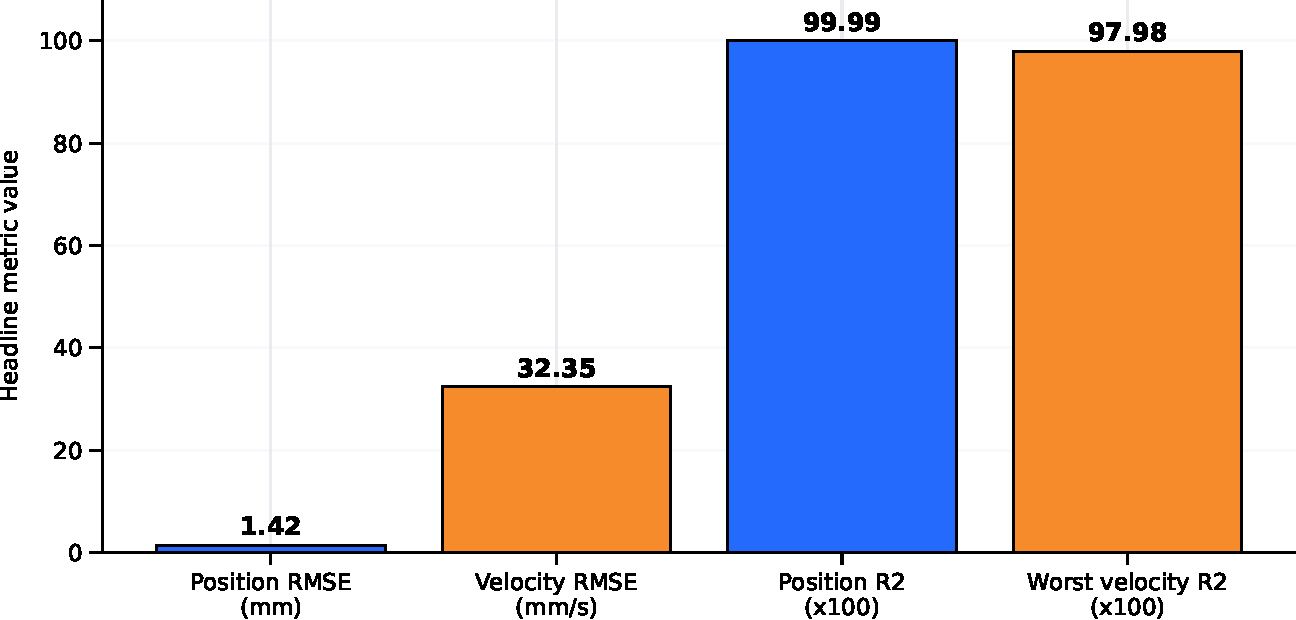
\includegraphics[width=.9\textwidth]{figures/result_summary.pdf}\caption{Headline translation-only metrics. Position is essentially exact at the rendered scale; velocity is accurate but has a larger and direction-dependent residual.}\label{fig:summary}\end{figure}
The millimetric position error is consistent with a coordinate-aware encoder followed by a keypoint-like spatial bottleneck. Velocity is harder because it depends on differences over a \,10 ms interval. Small visual localization errors are divided by a small $\dt$, amplifying rate noise. A simple propagation argument illustrates the scale:
\begin{equation}
\delta v\approx\frac{\sqrt{2}\,\delta p}{\dt}.
\end{equation}
With $\delta p$ at the millimetre level and $\dt=0.01$ s, naive differencing alone could yield errors on the order of tenths of metres per second. The learned spatial motion encoder reduces this substantially, but the principle explains why velocity remains the more difficult output.

\subsection{Layer-wise representation probes}
\begin{figure}[htbp]\centering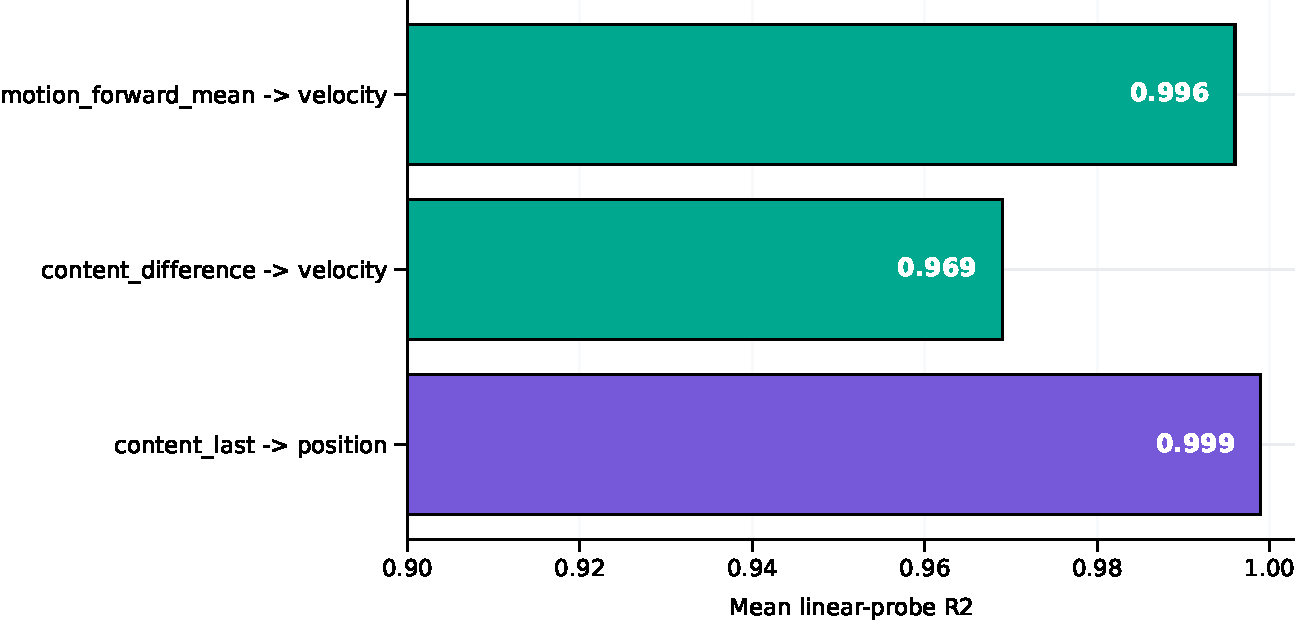
\includegraphics[width=.9\textwidth]{figures/probe_results.pdf}\caption{Selected linear-probe results. Values summarize mean $R^2$ across physical components.}\label{fig:probes}\end{figure}
The content latent permits almost perfect linear position decoding ($R^2\approx0.999$), while the motion-forward mean permits nearly linear velocity decoding ($R^2\approx0.996$). The difference between adjacent content embeddings already carries substantial velocity information ($R^2\approx0.969$). These observations support, but do not prove, a configuration/tangent interpretation:
\begin{equation}
\bm z_t\sim\text{configuration-like coordinates},\qquad
\bm m_t\sim\text{tangent-like coordinates}.
\end{equation}
The spatial-map mean has an effective rank near 1.22 in the evaluation statistics. This should not be read as the rank of the full spatial tensor: spatial averaging can discard precisely the location-dependent variation the encoder was designed to preserve. It may indicate a compact global summary, or it may expose an axis-selective bottleneck. Channel-wise and spatially resolved singular spectra are needed to distinguish these hypotheses.

\subsection{Intervention results}
\begin{figure}[htbp]\centering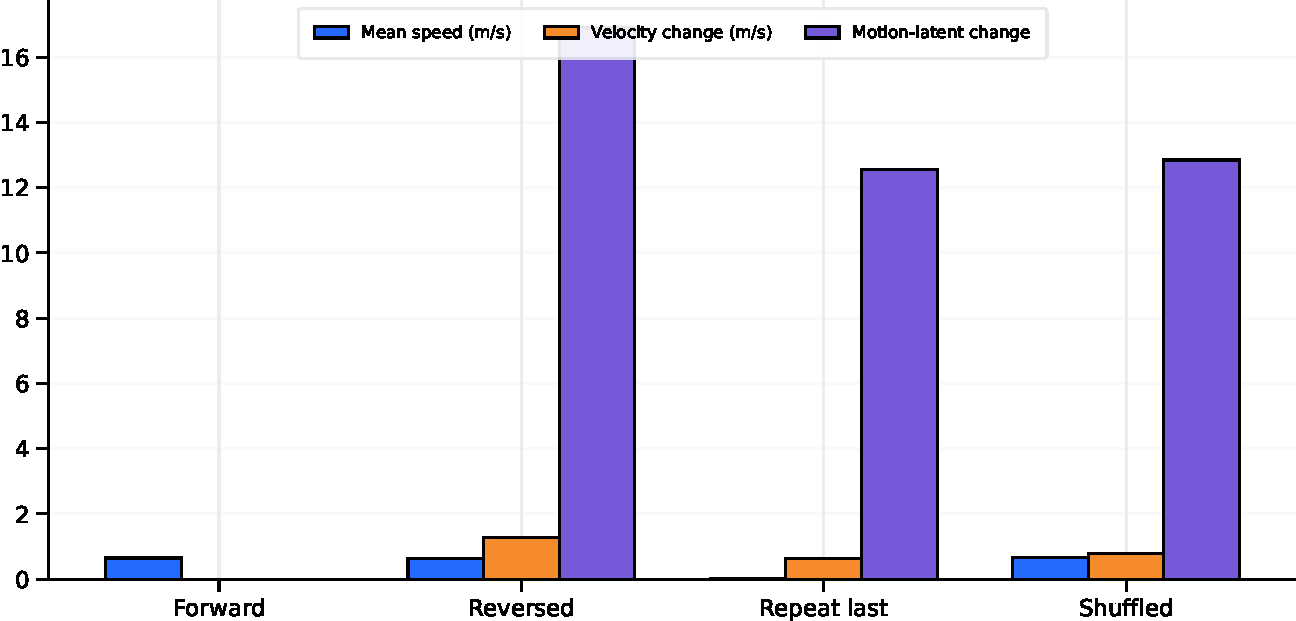
\includegraphics[width=.9\textwidth]{figures/interventions.pdf}\caption{Temporal intervention summary. Repeating a static frame suppresses predicted speed; reversing the sequence significantly changes and approximately reverses velocity.}\label{fig:interventions}\end{figure}
The baseline mean predicted speed is approximately \,0.645 m/s. Repeating the last frame produces only \,0.012 m/s, strong evidence that velocity depends on temporal change. Reversal changes velocity by approximately \,1.286 m/s, close to twice the baseline speed as expected for sign reversal, and the reported reversal error is about \,0.062 m/s. Shuffling substantially alters motion latents and velocity while retaining approximately the same speed scale, indicating sensitivity to local temporal order rather than only overall frame content.

\subsection{Why the results look this way}
\begin{enumerate}
\item \textbf{Position is easiest because absolute coordinates are explicit.} Coordinate channels expose image location, the feature map maintains spatial organization, and the keypoint readout computes differentiable expected coordinates.
\item \textbf{Velocity benefits from pre-pooling temporal structure.} The motion encoder sees $\bm F_t$, $\bm F_{t+1}$, and normalized feature rate on a $16\times16$ grid. It can suppress static background and combine local changes before global compression.
\item \textbf{The head assignment encourages factorization.} Position is read from $\bm z_t$ alone; velocity receives endpoint content and $\bm m_t$. This asymmetric information route makes a position-heavy content latent and velocity-heavy motion latent an economical solution.
\item \textbf{Bidirectionality injects a physical symmetry.} Time reversal encourages velocity sign inversion and makes temporal direction testable.
\item \textbf{Metric correction improves coherence but cannot repair all perception errors.} The physical corrector adjusts decoded trajectories locally. It does not alter the visual representation, so systematic visual ambiguities or axis-dependent calibration remain upstream.
\item \textbf{Higher-speed cases are less forgiving.} Faster motion causes larger inter-frame displacement and may challenge receptive-field correspondences, heatmap smoothness, and the first-order latent transition.
\end{enumerate}

\section{Feature maps, keypoints, and Slot Attention}
A feature map is a per-location representation. Soft keypoints transform it into a small set of landmark statistics. Slot Attention instead uses iterative competitive attention to produce exchangeable per-object vectors \cite{locatello2020slot}. The correspondence is summarized as
\begin{equation}
\underbrace{\bm F_t[i,j]}_{\text{per spatial location}}
\longrightarrow
\underbrace{\bm k_t^{(1:K)}}_{\text{per learned landmark}}
\quad\text{versus}\quad
\underbrace{\bm F_t[i,j]}_{\text{per spatial location}}
\longrightarrow
\underbrace{\bm s_t^{(1:K)}}_{\text{per object slot}}.
\end{equation}
For a single ball, keypoints are appropriate because several landmarks can jointly estimate pose and appearance without solving object assignment. For multiple balls, variable object counts, or interactions, a slot-based or set-based architecture would provide a more natural entity decomposition.

\section{Ablations and diagnostic experiments}
The following experiments would most efficiently test the architectural explanations.
\begin{longtable}{p{0.25\textwidth}p{0.32\textwidth}p{0.34\textwidth}}\toprule
Ablation & Question & Expected diagnostic \\\midrule\endhead
Remove coordinate channels & Is absolute localization learned from content or background shortcuts? & Position error should rise, especially under camera/background changes.\\
Replace keypoints by global average pooling & Does structured localization explain position precision? & Position probes and metric accuracy should degrade; appearance invariance may improve.\\
Compute motion from $\bm z_{t+1}-\bm z_t$ only & Is spatial pre-pooling differencing essential? & Velocity error should increase if spatial correspondences matter.\\
Remove feature-rate normalization & Is optimization sensitive to $1/\dt$ scaling? & Training instability or speed-dependent bias may emerge.\\
Remove reversal loss & Does bidirectional symmetry cause sign-correct reversal? & Reversal error should worsen more than forward RMSE.\\
Set refinement iterations to $0,1,2,4,8$ & Is the corrector genuinely iterative and stable? & Plot kinematic residual and state RMSE versus iteration.\\
Remove physics corrector but retain kinematic loss & Separate training regularization from inference refinement. & Reveals whether gains arise in representation or post-processing.\\
Randomize $\dt$ during training & Does the model learn rate rather than frame displacement? & Better transfer across frame rates would support physical scaling.\\
Spatially resolved SVD & Is low effective rank an averaging artifact? & Compare spectra of flattened $C\times HW$, channel means, and keypoints.\\
Background/camera intervention & Is position encoded geometrically or through environmental cues? & Stable performance under texture changes supports genuine object localization.\\\bottomrule
\end{longtable}

\section{Recommended architecture extensions}
\subsection{Autonomous prediction}
To obtain open-loop rollout, introduce a recurrent dynamic state $\bm s_t=[\bm z_t;\bm m_t]$:
\begin{equation}
\widehat{\bm s}_{t+1}=G_\theta(\bm s_t,\dt),\qquad
(\widehat{\bm p}_{t+1},\widehat{\bm v}_{t+1})=H_\theta(\widehat{\bm s}_{t+1}).
\end{equation}
For translation-only free flight, an interpretable baseline should always be included:
\begin{equation}
\widehat{\bm p}_{t+k}=\widehat{\bm p}_t+k\dt\widehat{\bm v}_t,
\qquad \widehat{\bm v}_{t+k}=\widehat{\bm v}_t.
\end{equation}
The learned rollout should be compared against this observer-plus-physics baseline, not only against persistence.

\subsection{Hybrid latent refinement}
A case-independent corrector should refine both content and motion, then retain a decoded physical residual:
\begin{align}
(\bm z^{(k+1)},\bm m^{(k+1)})&=\mathcal C_z(\bm z^{(k)},\bm m^{(k)},\bm r_z^{(k)}),\\
(\bm p,\bm v)&=H(\bm z^{(K)},\bm m^{(K)}),\\
\bm r_p&=\bm p_{t+1}-\bm p_t-\dt\bm v_t.
\end{align}
This retains generality while preserving an interpretable metric anchor.

\subsection{Object-centric multi-body extension}
For multiple bodies, replace the single global content vector by a set of entity states:
\begin{equation}
\mathcal S_t=\{\bm s_t^1,\ldots,\bm s_t^N\},
\end{equation}
and model interactions with attention or a graph network. Slot Attention is one possible front end, but temporal slot identity and collision/contact assignment must be handled explicitly.

\section{Threats to validity}
\begin{itemize}
\item The reported experiment is translation-only and successful; conclusions may not transfer to rotation, combined motion, contacts, occlusion, or real imagery.
\item Linear decodability is not causal disentanglement. Correlated factors can be linearly recoverable from the same representation.
\item The effective-rank statistic depends strongly on which axes are flattened or averaged.
\item One-step latent prediction does not establish stable long-horizon rollout.
\item Simulator labels and rendering calibration may make the task easier than real visual state estimation.
\item A fixed frame rate allows the network to exploit displacement scale. Frame-rate variation is needed to establish genuine rate awareness.
\item The iterative corrector may be trained only for a fixed number of unrolled steps; convergence outside that regime is unproven.
\end{itemize}

\section{Reproducibility checklist}
\begin{enumerate}
\item Preserve trajectory-level train/validation/test separation and fixed seeds.
\item Record exact normalization statistics for images, feature rates, positions, and velocities.
\item Save both raw and corrected outputs to separate correction effects from observer effects.
\item Report errors by axis, speed, image location, and trajectory.
\item Export feature maps, keypoint heatmaps, keypoint confidence, $\bm z_t$, $\bm m_t$, latent residuals, and physical residuals.
\item Evaluate forward, reverse, repeat-last, shuffle, and frame-rate interventions.
\item Report probe train/test separation and regularization to avoid optimistic linear probes.
\item Sweep refinement steps at evaluation while plotting residual monotonicity.
\item Compare against direct CNN-to-state, global-pooling, optical-flow, and observer-plus-analytic-rollout baselines.
\end{enumerate}

\section{Conclusion}
The architecture's strong translation-only performance is consistent with a coherent chain of inductive biases. Coordinate augmentation makes absolute position accessible; spatial feature maps preserve localization and motion evidence; soft keypoints create a compact geometric description; separate content and motion pathways encourage a configuration/tangent split; latent prediction organizes adjacent representations; reversal consistency encodes temporal parity; and metric-space refinement reduces kinematic inconsistency. The results support this interpretation through excellent position accuracy, strong velocity accuracy, linearly decodable position and velocity in different representation stages, and appropriate responses to temporal interventions. The model should nevertheless be called a neural observer with local predictive structure until autonomous multi-step rollout is implemented and evaluated.

\appendix
\section{Tensor-shape reference}
\begin{table}[htbp]\centering
\begin{tabularx}{\textwidth}{lXl}\toprule
Symbol & Meaning & Shape \\\midrule
$\bm I$ & RGB window & $B\times T\times3\times256\times256$\\
$\widetilde{\bm I}$ & RGB plus coordinate channels & $B\times T\times5\times256\times256$\\
$\bm F$ & final spatial feature maps & $B\times T\times128\times16\times16$\\
$\bm k$ & soft-keypoint descriptor & $B\times T\times168$\\
$\bm z$ & content embeddings & $B\times T\times256$\\
$\Delta\bm F$ & adjacent feature differences & $B\times(T-1)\times128\times16\times16$\\
$\bm U$ & motion-encoder spatial input & $B\times(T-1)\times384\times16\times16$\\
$\bm m$ & interval motion embeddings & $B\times(T-1)\times256$\\
$\bm q$ & velocity-head input & $B\times(T-1)\times768$\\
$\widehat{\bm p}$ & position estimate & $B\times T\times3$\\
$\widehat{\bm v}$ & frame-wise velocity estimate & $B\times T\times3$\\\bottomrule
\end{tabularx}
\end{table}

\section{Key implementation facts}
\begin{verbatim}
image:              256 x 256 x 3, ImageNet normalization
coordinate input:   2 channels, each in [-1, 1]
context:            10 frames at 100 Hz
backbone channels:  5 -> 32 -> 64 -> 128 -> 128
backbone resolution:256 -> 128 -> 64 -> 32 -> 16
soft keypoints:     8, with 16 appearance values each
content dimension:  256
motion dimension:   256
velocity input:     [z_t, z_(t+1), m_t] = 768 dimensions
optimizer config:   learning rate 3e-4, weight decay 0.05
training:           75 epochs, bf16 mixed precision, grad clip 1.0
\end{verbatim}

\bibliographystyle{plain}
\bibliography{references}
\end{document}
